% =======================================================================
% =                                                                     =
% =======================================================================
% -----------------------------------------------------------------------
% - Author:     Chaua Queirolo                                          -
% - Version:    001                                                     -
% -----------------------------------------------------------------------
\documentclass[a4paper,11pt]{article}    

% =======================================================================
% PACKAGES
% =======================================================================

% Language support
\usepackage[brazil]{babel}
\usepackage[utf8]{inputenc}
\usepackage[T1]{fontenc}
\usepackage{ae,aecompl}

% Configuration
\usepackage{url}
\usepackage{enumerate}
\usepackage{color}
\usepackage[svgnames,table]{xcolor}
\usepackage[margin=2cm,includefoot]{geometry}

% Tabular
\usepackage{multirow}
\usepackage{multicol}

% Images
\usepackage{graphicx}
\usepackage[scriptsize]{subfigure}
\usepackage{epstopdf}
\usepackage{float}% http://ctan.org/pkg/{multicol,lipsum,graphicx,float}

% Math
\usepackage{mdwtab}	% bug rowcolor
\usepackage{amssymb}
\usepackage{amsmath}
\usepackage{footnote}

% References
\usepackage[sort,nocompress]{cite}

% =======================================================================
% VARIABLES
% =======================================================================

% Space between the lines in a table
\renewcommand{\arraystretch}{1.3}

% Define a new column type
\newcolumntype{x}[1]{>{\raggedright\hspace{0pt}}p{#1}}%

% Controle das Margens
\sloppy
\tolerance=9999999

% Espaço entre colunas
\setlength{\columnsep}{.9cm}


% Configuration
\usepackage{lipsum}
\usepackage{blindtext}

% =======================================================================
% HEADER
% =======================================================================

\title{Algoritmos Genéticos}
\author{Gabriel Pinto Ribeiro da Fonseca\\E-mail: {\tt gabriel-prdf@hotmail.com}}
\date{}

\newenvironment{Figure}
  {\par\medskip\noindent\minipage{\linewidth}}
    {\endminipage\par\medskip}

% =======================================================================
% DOCUMENT
% =======================================================================
\begin{document}

\maketitle


\begin{multicols}{2}
\section{Introdução}
Ao se obter um problema de otimização ou busca, ele e composto por três componentes principais, a codificação do problema, a função objetivo que procura a maximizar ou minimizar e o espaço de soluções associado \cite{ref:marcio2009b}.
 Os Algoritmos genéticos auxiliam na solução destes problemas.
 
 Os algoritmos genéticos foram concebidos em 1960 por John Holland, tendo como motivo estudar os fenômenos relacionados a adaptação e seleção das especes junto a natureza, e implementá-las em algorítimos \cite{ref:aurora2004b}.

\section{Descrição do algoritmo genético e estratégia evolutivas}
O algoritmo genético é composto pelos cromossomos, população, geração, fitness, filhos e mutação.
\begin{enumerate}
\item Cromossomo é a cadeia de bits que representam as características, representando assim uma solução possível.
\item População é o grupo de indivíduos que deles se obtêm a solução desejada, efetuando cruzamentos de características.
\item Geração é a iteração completa do algoritmo genético para criação de uma nova população(filhos).
\item Fitness é o valor que o cromossomo possui, este valor e sua avaliação para o problema.
\item Filhos são a nova população obtida pela geração.
\item Mutação é a responsável por obter características que podem melhorar a solução e impedir que a população se torne igual rapidamente.
\end{enumerate}

\begin{enumerate}
\item Inicialização da população
\item Calcula-se o fitness de cada indivíduos
\item Selecionado os indivíduos para reprodução
\item Cruzamento (podendo sofrer mutação)
\item Volta ao passo 3 e efetua os procedimentos novamente, até ser encontrada a solução desejada.
\end{enumerate}
O algoritmo genético inicia-se com a população incial, esta populacao pode ser criada de forma aleatória, pois caso não seja, pode ocorrer um problema de conversão rapida, queria a obtenção de uma solução que não é a correta, e de forma que nao se pode obter outra solução.

O calculo do fitness é determinado pelo problema, o desenvolvedor que deve criar a função de aptidao para se dar o valor ao cromossomo, podendo se obter o maximo ou minimo para a solução final.

A seleção dos individuos para a reprodução pode ocorre por varios metodos, dois deles são a seleção por torneio e a seleção por roleta. 

No cruzamento ocorre a troca de dados dos pais, para gerar assim um novo cromossomo, este cromossomo em criação pode sofrer um mutação no processo, algumas das técnicas utilizadas neste passo e o ponto de corte.

\subsection{Torneio}
A seleção pela técnica de torneio, ocorre com a seleção aleatória de cromossomos, onde estes competiram entre eles, e o indivíduo com o maior cromossomos e escolhido. Após este passo, os competidores são recolocados na população, e é efetuado um novo sorteio para mais uma competição, este processo e repedido até não ser mais necessário.\cite{ref:oliveira2004b}

%A figura abaixo, ilustra o funcionamento do torneio.

\begin{figure}[!htb]
	\centering
	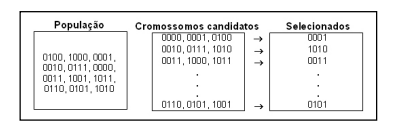
\includegraphics{imagens/torneio}
\end{figure}

\subsection{Roleta}
A seleção pela técnica de roleta, ocorre de forma proporcional ao valor de fitness de cada cromossomo, sendo representados em uma roleta, sua representação na roleta é de acordo com a sua relevância(fitness), quanto maior for, maior o espaço terá nela \cite{ref:oliveira2009}.
Após ter a roleta pronta, é usada de forma aleatória para se obter os pais selecionados

%A figura abaixo ilustra o formato da roleta, e exemplifica para melhor compreenção.
\begin{figure}[!htb]
	\centering
	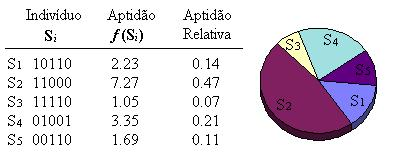
\includegraphics{imagens/roleta.jpg}
\end{figure}



\subsection{Ponto de core}
Neste metodo de cruzamento, com os pais já selecionados, é escolhido um ponto de corte, do inicio do pai1 até o ponto de corte e dado ao filho1, e do ponto de corte no pai2 ao fim é completado o filho1, este procedimento e feito o inverso com o filho 2.

%A imagem a baixo ilustra o processo.
\begin{figure}[!htb]
	\centering
	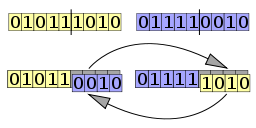
\includegraphics{imagens/corteUnico}
\end{figure}


Utilizando este mesmo conceito, tem-se a tecnica de multi corte, podendo ser de dois corte ao quanto desejar, seu funcionamento e identico ao de corte unico descrito acima. É efetuado varios cortes, e distribuidos aos filhos.

%A imagem abaixo ilustra os cortes realizados, e o filho gerado.
\begin{figure}[!htb]
	\centering
	\includegraphics{imagens/corteMult}
\end{figure}

\section{Exemplos de aplicações}
Sistemas que possuem um bom desempenho em um ambiente dinâmico, exigem uma solução que se adapte, com esta característica, torna-se mais fácil resolver as questões impostas a ele\cite{ref:andre2009b}. O algoritmo genético é muito utilizado em ambientes que tem esta necessidade, que são por natureza complexos, como seleção de rotas, problemas de otimização, engenharia de sistemas neurais artificiais, evolução interna de imagens, entre outros.


\subsection{Conclusão}
Com o algoritmo genético, é possivel obter soluções que exigem uma evolução constante, utilizando como logica o funcionameno genetico, e tendo uma ama grande de tecnicas para se procurar a melhor solução.

\bibliographystyle{plain}
\bibliography{referencias}

\end{multicols}
\end{document}

